\scanpage{31}
\margin{30}

Considérons un graphe comb. $\Gamma=(S,\vec A,\sigma_0,\unsure{\alpha})$ avec une semi-circularisation (structure polygonale \inserted{donnée} sur l'ens des sommets issus d'une \unsure{arête} donnée) et \deleted{pour tout} d'isom de transport
\[
\varphi_{\vec a}:\underbrace{\omega(\vec A_s)}_{\omega_s}\mathbin{-}\underbrace{\omega(\vec A_t)}_{\omega_t}\qquad\text{pour }\vec a:s\longrightarrow t
\]
(satisfaisant la seule condition
\[
\varphi_{-\vec a}=\varphi_{\vec a}^{-1}
\]
)

On suppose pour simplifier que les ordres des sommets sont $\ge3$ (sinon il faut se donner, pour les sommets d'ordre $1\le\nu\le2$, une structure de polygône combinatoire ayant $\vec A_s$ comme ens des sommets, i.e. avec un ens de deux orientations, de façon à pouvoir \unsure{en tenir} à la donnée des $\varphi_{\vec a}$). La surface associée aux $\varphi_{\vec a}$ est obtenue ainsi : on considère la réalisation topologique canonique \inserted{par disque polygonal} du polygône dual de chaque $\vec A_s$ (ce qui peut se faire via une décomposition barycentrique de $\overline A_s$, qui donne une réalisation simultanée pour \deleted{les deux} $\overline A_s$ et pour le polygône dual, chaque réalisation $\operatorname{Dis}_s$ apparaissant comme réunion de $2\nu_s$ \uline{drapeaux} correspondant aux repères de $\vec A_s$ --- i.e. les arêtes de ces polygônes correspondent aux \deleted{faces} \inserted{sommets} de $\vec A_s$, i.e. aux arêtes \deleted{\unsure{de}} de $\Gamma$ \deleted{\unsure{d'}} d'origine $s$.

\margin{cas $\nu_s=1,2$ n'est pas exclu}

\figure{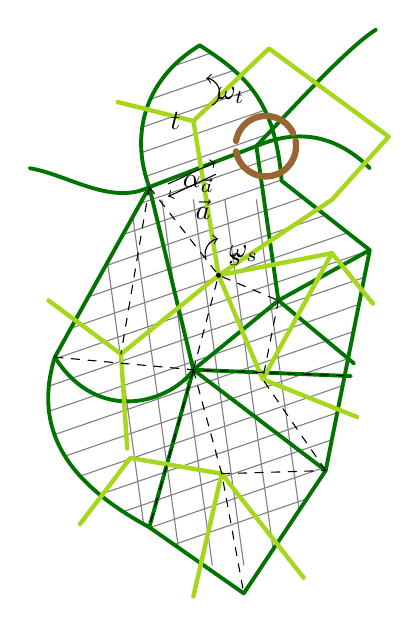
\begin{tikzpicture}[x=.8cm,y=.8cm,line cap=round,line join=round]
\begin{scope}\clip (-2,-.7)..controls(-2.4,-2)and(-1.6,-2.8)..(-.5,-3.4)--(1,-4.45)--(2.3,-2.5)--(3,1)--(1.6,2.1)..controls(1.5,3.4)and(1,3.8)..(.3,4.25)..controls(-.6,3.7)and(-.8,2.8)..(-.5,2)--cycle;
\foreach \y in {-4.5,-4.1,...,4}{\draw[gray] (-2.5,\y)--(3.3,{\y+2});}\foreach \x in {-.5,0,.5,1,1.5,2}{\draw[gray] (\x,-4)--({\x-.8},1.8);}\end{scope}
\draw[green!45!black,line width=1.4pt] (-2,-.7)..controls(-2.4,-2)and(-1.6,-2.8)..(-.5,-3.4)--(1,-4.45)--(2.3,-2.5)--(3,1)--(1.6,2.1)..controls(1.5,3.4)and(1,3.8)..(.3,4.25)..controls(-.6,3.7)and(-.8,2.8)..(-.5,2)--cycle;
\draw[green!45!black,line width=1.4pt] (-2,-.7)..controls(-1.3,-1.8)and(-.15,-1.4)..(.2,-.9)--(1.55,.2)--(3,1);
\draw[green!45!black,line width=1.4pt] (-.5,-3.4)--(.2,-.9)--(-.5,2)--(1.2,2.65)..controls(2,3)and(2.6,2.7)..(3,2.3);
\draw[green!45!black,line width=1.4pt] (.2,-.9)--(2.3,-2.5) (.2,-.9)--(2.7,-1) (1.2,2.65)--(1.55,.2)--(2.75,-.8);
\draw[green!45!black,line width=1.4pt] (1.2,2.65)..controls(2,3.5)and(2.7,4.25)..(3.1,4.5) (-.5,2)..controls(-1.1,1.7)and(-1.8,2.2)..(-2.4,2.3);
\draw[yellow!65!green,line width=1.6pt] (-1.6,-3.35)--(-.8,-2.3)--(.65,-2.55)--(1.95,-4.2) (.65,-2.55)--(.2,-4.5);
\draw[yellow!65!green,line width=1.6pt] (-2.1,.2)--(-.95,-.65)--(-.85,-2.15) (-.95,-.65)--(.6,.6)--(2.4,.95)--(3.05,.15);
\draw[yellow!65!green,line width=1.6pt] (-1,3.35)--(.2,3.05)--(.6,.6)--(1.3,-1.05)--(2.4,.95) (1.3,-1.05)--(2.8,-1.65);
\draw[yellow!65!green,line width=1.6pt] (.2,3.05)--(1.4,4.2)--(3.3,2.8)--(2.4,1.8)--(.6,.6);
\draw[dashed] (-2,-.7)--(.2,-.9)--(2.7,-1) (-.5,2)--(.6,.6)--(1.55,.2) (-.5,2)--(-.95,-.65) (.2,-.9)--(.6,.6) (.2,-.9)--(-.5,-3.4) (.2,-.9)--(.65,-2.55)--(1,-4.45) (.65,-2.55)--(2.3,-2.5) (1.55,.2)--(1.3,-1.05)--(2.3,-2.5);
\draw[brown!80!black,line width=2.3pt] (1.35,2.65) ++(10:.48) arc(10:-170:.48);\draw[brown!80!black,line width=2.3pt] (1.35,2.65) ++(25:.48) arc(25:170:.48);
\fill (.6,.6) circle(.04);\node[above right]at(.6,.6){$s$};\node[left]at(.15,3.05){$t$};
\draw[->] (.4,.85) arc(200:100:.25);\node at(1,.95){$\omega_s$};\draw[->] (.5,3.3) arc(-60:85:.23);\node at(.8,3.45){$\omega_t$};
\draw[->] (-.2,2.05)--(.55,2.4);\draw[<-] (-.2,1.85)--(.55,2.2);\node at(.35,1.65){$\vec a$};\node at(.28,2.05){$\unsure{\alpha_{\vec a}}$};
\end{tikzpicture}}

Ceci dit, on \uline{recolle}, pour tte $\vec a\in\vec A$ \deleted{$\unsure{\sigma_0}$}, posant $s=\operatorname{or}(\vec a)$, $t=\operatorname{ex}(\vec a)=\operatorname{or}(\unsure{\sigma\vec a|\alpha\vec a})$, \deleted{l'arête de $\operatorname{Dis}_s$} l'arête $\alpha_{\vec a}$ de $\operatorname{Dis}_s$ correspondant à $\vec a$, avec l'arête $\alpha_{-\vec a}$ de $\operatorname{Dis}_t$ correspondant à $-\vec a$, moyennant un isom \deleted{linéaire} \inserted{affine} sur les arêtes (donc défini \deleted{\unsure{par le choix}} d'une bijection sur les ens d'extrémités) \deleted{\unsure{avec le choix qui est donné}} \inserted{dont le choix est déterminé} à l'aide de l'isom de transport $\varphi_{\vec a}$ : la vérité, c'est que si les orientations $\omega_s$ de \deleted{$\operatorname{Dis}_s$} $\unsure{\vec A_s|\overline A_s}$, i.e. de $\operatorname{Dis}_s$, et $\omega_t$ de $\unsure{\vec A_t|\overline A_t}$, i.e. de $\operatorname{Dis}_t$, se correspondent, alors l'isom d'identification
\[
\psi_{\vec a}:\alpha_{\vec a}\xrightarrow{\sim}\alpha_{-\vec a}
\]
doit \deleted{\unsure{préserver}} \uline{renverser} les orientations induites par $\omega_s$ sur $\alpha_{\vec a}$ resp. $\omega_t$ sur $\alpha_{-\vec a}$.
